\documentclass{standalone}

\usepackage[euler-digits]{eulervm}

\usepackage{tikz}
\tikzset{every node/.style={circle,draw=none,minimum size=6mm,inner sep=0pt}}
\tikzset{t/.style={rectangle}}

\begin{document}
    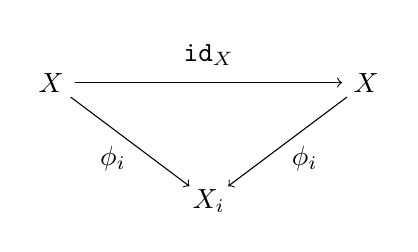
\begin{tikzpicture}[font=\sffamily]
      \node (i) at (0,-1.5) {$X_i$};
      \node (X+) at (2,0) {$X$};
      \node (X-) at (-2,0) {$X$};
        \draw[->] (X+) -- node[below right] {$\phi_i$} (i);
        \draw[->] (X-) -- node[below left] {$\phi_i$} (i);
        \draw[->] (X-) -- node[above] {$\mathtt{id}_X$} (X+);
    \end{tikzpicture}
\end{document}
